\documentclass[../main.tex]{subfiles}

\graphicspath{{../images/}}

\begin{document}
\pagestyle{fancy}
\lhead{Lecture 3: 1/23}
\chead{Chapter 3}
\rhead{PHYS 472}

\section*{Chapter 3: Crystal Binding and Elastic Constants}
\addcontentsline{toc}{section}{Chapter 3: Crystal Binding and Elastic Constants}

We are mostly interested in the E\&M interaction between atoms on the energy scale of eV (e.g. the
band gap of silicon is 1.2 eV). 

\paragraph{There are 4 main types of bonds:}

\subparagraph*{Metallic Bond} Bonds between metals have weakly bound valence electrons. Hence the
electrons move freely around like a fluid. This is why metals are good conductors.

\subparagraph*{Ionic Bond} Bonds between metals and non-metals (e.g. NaCl). The opposing charges
attract each other where the electrons form full shells and hence less conductivity.

\subparagraph*{Covalent Bond} Bonds between non-metals (e.g. Si). The atomic orbitals defined by
QM describes the bonds through the hybridization of the orbital wavefunctions (e.g. $sp^3$ in
diamond). This is a very difficult problem to solve.

\subparagraph*{Van der Waals interaction} Inert gases... e.g. He is interesting as it is a liquid at
very low temperatures, and it is a boson (He-4 superfluid) and fermion (He-3) depending on the
number of neutrons. 

\subparagraph*{Hydrogen Bonding} is very important in biology, but not in solid state physics.

\subsection*{Van der Waals interaction}

Two types of energy to consider:
\begin{itemize}
\item Cohesive energy: Energy required to separate bound atoms. The cohesive energy of a solid
is the sum of the cohesive energies of the bonds. 
\item Ionization energy: Energy required to remove an electron from an atom.
\end{itemize}

The ionization energy is larger because the Van der Waals interaction is a weaker bond. Given two
inert gas atoms, there is no dipole or charge distribution contributing to the interactions between
the atoms. In QM, there is no zero point energy, so we have to consider the atoms to not be perfect,
but rather vibrate around a mean position. This is a dipole-dipole interaction. 

\paragraph{dipole-dipole }Given two electrons spaced by a distance $R$ in a 1D lattice, one atom
fluxuates by $x_2$ and the other by $x_1$. The Hamiltonian of the unpertubed system is
\begin{align*}
    H_o = \frac{p_1^2}{2m} + \frac{p_2^2}{2m} + \frac{1}{2} C x_1^2 + \frac{1}{2} C x_2^2
\end{align*}
The Coulomb interaction:
\begin{align*}
    H_1 = \frac{e^2}{R} + \frac{e^2}{R + x_1 - x_2} - \frac{e^2}{R + x_1} - \frac{e^2}{R - x_2}
\end{align*}
Using Taylor expansion (2nd order) for small $x_1$ and $x_2$ we get
\begin{align*}
    H_1 = -\frac{2e^2}{R^3} x_1 x_2
\end{align*}
Since this has 2 degrees of freedom, we have a 2x2 matrix with 2 eigenvalues diagonlized by the
normal mode transform. This results in 2 Canconical Modes:
\begin{align*}
    x_s = \frac{1}{\sqrt{2}}(x_1 + x_2) \quad x_a = \frac{1}{\sqrt{2}}(x_1 - x_2)
\end{align*}
THe total Hamiltonian is
\begin{align*}
    H &= \frac{1}{2m} \qt[\frac{1}{2}(p_s + p_a)^2] + \frac{1}{2m}\qt[\frac{1}{2}(p_s - p_a)^2]
    - 2 \frac{e^2}{R^3} \cdot \frac{1}{2} (x_s^2 - x_a^2) + \frac{1}{2} cx_1^2 + \frac{1}{2} cx_2^2\\
    &= \qt[\frac{p_s}{2m} + \frac{1}{2} \qt(c - \frac{2e^2}{R^3})x_s^2] +
    \qt[\frac{p_a}{2m} + \frac{1}{2} \qt(c + \frac{2e^2}{R^3})x_a^2]
\end{align*}

\pagebreak
\lhead{Lecture 4: 1/25}

\section*{Chapter 3: cont'd}

The momenta of the harmonic oscillators from last time are also in the ofmr 2 modes:
\begin{align*}
    p_s = \frac{1}{\sqrt{2}}(p_1 + p_2) \quad p_a = \frac{1}{\sqrt{2}}(p_1 - p_2)
\end{align*}
The matrix form
\begin{align*}
    \begin{pmatrix}
        E_o & 0 \\
        0 & E_o
    \end{pmatrix} \mqty(a \\ b)
    = \hbar \omega \mqty(a \\ b)
\end{align*}
\begin{align*}
    \begin{vmatrix}
        E_o - \hbar \omega & \Delta \\
        \Delta & E_o - \hbar \omega
    \end{vmatrix}
    = 0
\end{align*}
solving for the eigenstates
\begin{align*}
    \frac{1}{\sqrt{2}} \mqty(a \\ b), \quad \frac{1}{\sqrt{2}} \mqty(a \\ -b)
\end{align*}
The Hamiltonian of the single harmonic oscillator is
\begin{align*}
    H_o = \frac{p^2}{2m} + \frac{1}{2} m \omega^2 x^2
\end{align*}
thus we can compare the frequencies of the harmonic oscillator and the Van der Waals interaction
\begin{align*}
    \omega = \sqrt{\frac{c \pm \frac{2e^2}{R^3}}{m}}
\end{align*}
and we know the \emph{zero-point energy} $1/2 \hbar \omega$ or in this case 
\begin{align*}
    \frac{1}{2} \hbar \Delta \omega = \frac{1}{2} \hbar [\Delta \omega_s + \Delta \omega_a]
\end{align*}
From the uncoupled sum and using Taylor expansion
\begin{align*}
    \omega = \omega_o \qt[1 \pm \frac{1}{2} \qt(\frac{2e^2}{R^3c})
    \pm \frac{1}{8} \qt(\frac{2e^2}{R^3c})^2 + \dots]
\end{align*}
thus we ge the interaction energy
\begin{align*}
    \Delta U = \frac{1}{2} \hbar (\Delta \omega_s + \Delta \omega_a)
    = \frac{\hbar\omega_o}{2} \qt[\frac{e^4}{c^2 R^6}] = -\frac{A}{R^6}
\end{align*}
where the minus sign indicates an attractive force. We would expect the atoms to collapse, but
this is not the case due to the Pauli exclusion principle (electrons cannot occupy the same state).

\subsubsection*{Pauli exclusion principle}

As the atoms get closer, there is an overlap of the wavefunctions. If the wavefunctions are
symmetric, the spin states must be anti-symmetric. Therefore anti-symmetric wavefunctions have
symmetric spin states. This repulsive force from the Pauli exclusion principle is typically
found empirically $\propto \frac{1}{R^{12}}$. Therefore the total potential is
\begin{align*}
    U(R) = 4 \epsilon \qt[\qt(\frac{\sigma}{R})^{12} - \qt(\frac{\sigma}{R})^{6}]
\end{align*}
AKA the Lennard-Jones potential. We could find the equilibrium distance by minimizing the
potential $\dv{U}{R} = 0$. This is fine for inert gases that are spherical, but other molecules are
depend on more than the scalar distance $R$. This decays faster than the scale of Coulombs Law
$\propto \frac{1}{R^2}$. The total energy for a crystal is
\begin{align*}
    E = \frac{1}{2} N (4\epsilon) \qt[
        \sum_j ' \qt(\frac{\sigma}{P_{ij}R})^{12} - \sum_j ' \qt(\frac{\sigma}{P_{ij}R})^{6}
    ]
\end{align*}
where the prime indicates that the sum is over the nearest neighbors. The fcc lattice
\begin{align*}
    \sum_j' \qt(\frac{1}{P_{ij}})^{12} = 12.13188; \qquad \sum_j' \qt(\frac{1}{P_{ij}})^6 = 14.45392
\end{align*}
for the 12 nearest neighbors. Solving for the minimum energy $\dv{U}{R} = 0$ we get 
\begin{align*}
    R_o / \sigma = 1.09
\end{align*}

\subsubsection*{Ionic Crystal}

The Coulomb interaction: 
\begin{align*}
    \pm \frac{q^2}{r_{ij}}
\end{align*}
The short-term interaction 
\begin{align*}
    \lambda e^{-r_{ij}/\rho}
\end{align*}
thus the potential is
\begin{align*}
    U_{ij} = \lambda e^{-r_{ij}/\rho} \pm \frac{q^2}{r_{ij}}
\end{align*}
where at one site (one ion)
\begin{align*}
    U_i = \sum_j' U_{ij}
\end{align*}
and the total energy is
\begin{align*}
    U = N U_i
\end{align*}
For N molecules
\begin{align*}
    U_{ij} = \begin{cases}
        \lambda e^{-r_{ij}/\rho} - \frac{q^2}{r_{ij}} & \text{nearest neighbor} \\
        \pm \frac{q^2}{r_{ij}} & \text{otherwise}
    \end{cases}
\end{align*}
and the total energy is
\begin{align*}
    U_{tot} = N \qt[z e^{-R/\rho} - \alpha \frac{q^2}{R}] \qquad \alpha = \sum_j' \frac{\pm}{p_{ij}}
\end{align*}
where $z$ is the number of nearest neighbors, and $\alpha$ is the Madelung constant. From this we
can find the lattice constant by using
\begin{align*}
    \dv{U}{R} = 0 \rightarrow R_o^2 e^{-R_o/\rho} = \alpha \rho \frac{q^2}{z\lambda}
\end{align*}
solving for $R_o$ and putting into the total energy equation we get
\begin{align*}
    U_{tot} = -\frac{N\alpha q^2}{R_o} (1 - \frac{\rho}{R_o}) 
\end{align*}
where we have a special term
\begin{align*}
    -\frac{N\alpha q^2}{R_o}
\end{align*}
known as the `Madelung Energy'.

\pagebreak
\lhead{Lecture 5: 1/30}

\section*{Bonds Bonds and Bonds}
From last time:
\begin{align*}
    U_{ij} = \begin{cases}
        \lambda e^{-R/\rho} - \frac{q^2}{R} & \text{nearest neighbor} \\
        \pm \frac{q^2}{p_ijR} & \text{otherwise}
    \end{cases}
\end{align*}
where $p_{ij}R = r_{ij}$ and the total energy (sum) is
\begin{align*}
    U_{tot} = N \qt[z e^{-R/\rho} - \alpha \frac{q^2}{R}]
\end{align*}
where $z$ is the number of nearest neighbors, $N$ is the total ions, and $\alpha$ is the Madelung
constant:
\begin{align*}
    \alpha = \sum_j' \frac{\pm}{p_{ij}}
\end{align*}
At the equilibrium seperation
\begin{align*}
    \dv{U}{R} = 0 \rightarrow R_o^2 e^{-R_o/\rho} = \alpha \rho \frac{q^2}{z\lambda}
\end{align*}
$R_o$ is the equilibrium seperation (position). Substituting this back into the total energy we get
the empirical formal for the equilibrium energy (ground state):
\begin{align*}
    U_{tot} = -\frac{N\alpha q^2}{R_o} \qt(1 - \frac{\rho}{R_o})
\end{align*} 
where the first term outside the parenthesis is the Madelung energy
\begin{align*}
    -\frac{N\alpha q^2}{R_o}
\end{align*}
\paragraph{The Evaluation of Madelung Constant}
\begin{figure}[ht]
    \centering
    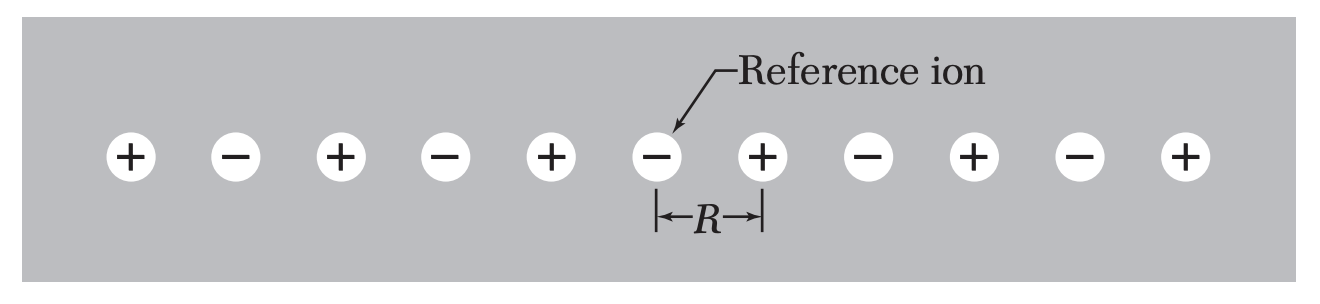
\includegraphics[width=0.4\linewidth]{ionline.png}
    \caption{Line of ions with alternating charges}
    \label{fig:4.1}
\end{figure}
Letting $R$ denote the distance between the ions, we can write the Madelung constant for the 1D line
of ions with alternating charges as.
\begin{align*}
    \frac{\alpha}{R} &= 2\qt[
        \frac{1}{R} - \frac{1}{2R} + \frac{1}{3R + \dots}
    ] \\
    &= \frac{2}{R} \qt[1 - \frac{1}{2} +...] \\
    \alpha &= 2 \ln{2} 
\end{align*}
Remember these numbers
\begin{itemize}
    \item Bohr radius $a_o = 0.529 {A}$
    \item fine structure constant $\alpha = \frac{e^2}{\hbar c} = \frac{1}{137}$
\end{itemize}
For the covalent bond, we have to use QM because the electron distribution is homogenous like
a sea of electrons. Sometimes we think of this as a homogenous electron gas. This is a very
difficult problem to solve. So we move on to the Hydrogen bond. This is a very weak bond typically
at the scale of meV--- room temperature is around 25 meV. So the bonds can break easily.

\end{document}